\chapter{Apêndices}

\section{Sistemas de Tempo Real}
São sistemas computacionais que dependem não somente que os dados computados estejam corretos, mas que sejam obtidos dentro de um intervalo de tempo 
pré determinado, que pode ser maior ou menor de acordo com a aplicação.
Na literatura, este período em que se espera que a resposta do sistema se dê é denominado \textit{deadline}.
Sistemas de tempo real podem ser classificados em dois tipos: \textit{soft} ou \textit{hard}.

Sistemas \textit{soft} são menos restritivos, tolerando eventuais perdas de \textit{deadline}; 
ao contrário dos sistemas \textit{hard}, em que estas perdas não são aceitáveis.  

Algumas características típicas, apesar de não obrigatórias, de sistemas de tempo real são limitações com relação ao tamanho, propósito específico e 
baixo custo \cite{silberschatz}.

\section{PWM}

\section{GFSK}

\section{banda ISM}

\section{SPI}

\section{CRC}
Método de detecção de erros aleatórios, isto é, de dados corrompidos ao longo do processo de transmissão ou armazenamento da informação por exemplo 
por ruídos, mas não por um agente \textquoteleft inteligente\textquoteright{} externo que modifique os dados transmitidos, tal qual um 
\textit{malware} \cite{stigge}.

Consiste essencialmente em uma divisão polinomial \cite{stigge}, logo, pode ser implementado em \textit{hardware}, utilizando-se apenas registradores 
de deslocamento com conexões realimentadas \cite{peterson}, assim como em \textit{software}. 
Em suma, trata-se de acrescentar à mensagem digital original um sufixo, que tem seu valor definido por operações realizadas em função da mensagem 
binária que intenta-se enviar e de um polinômio gerador.
Para o \textit{transceiver} nRF24L01+, dois polinômios geradores são utilizados: Eq. \ref{CRC_1} quando o dado cíclico adicionado é de 1 
\textit{byte} , e Eq. \ref{CRC_2}, para 2 \textit{bytes} \cite{nRF}.

Para uma descrição completa de como é implementado este método, vide \cite{stigge,peterson}.

\begin{equation}
\label{CRC_1}
G(X) = X^8 + X^2 + X + 1 
\end{equation}

\begin{equation}
\label{CRC_2}
G(X) = X^{16} + X^{12} + X^5 + 1 
\end{equation}

\section{MIFA} %% se der tempo, né?

\section{efeito hall} %% se der tempo, né?

\section{campo girante}

\section{\textit{schmitt trigger}}

\section{Diagrama da Classe RF24}
  \begin{figure}[!htb]
    \centering
    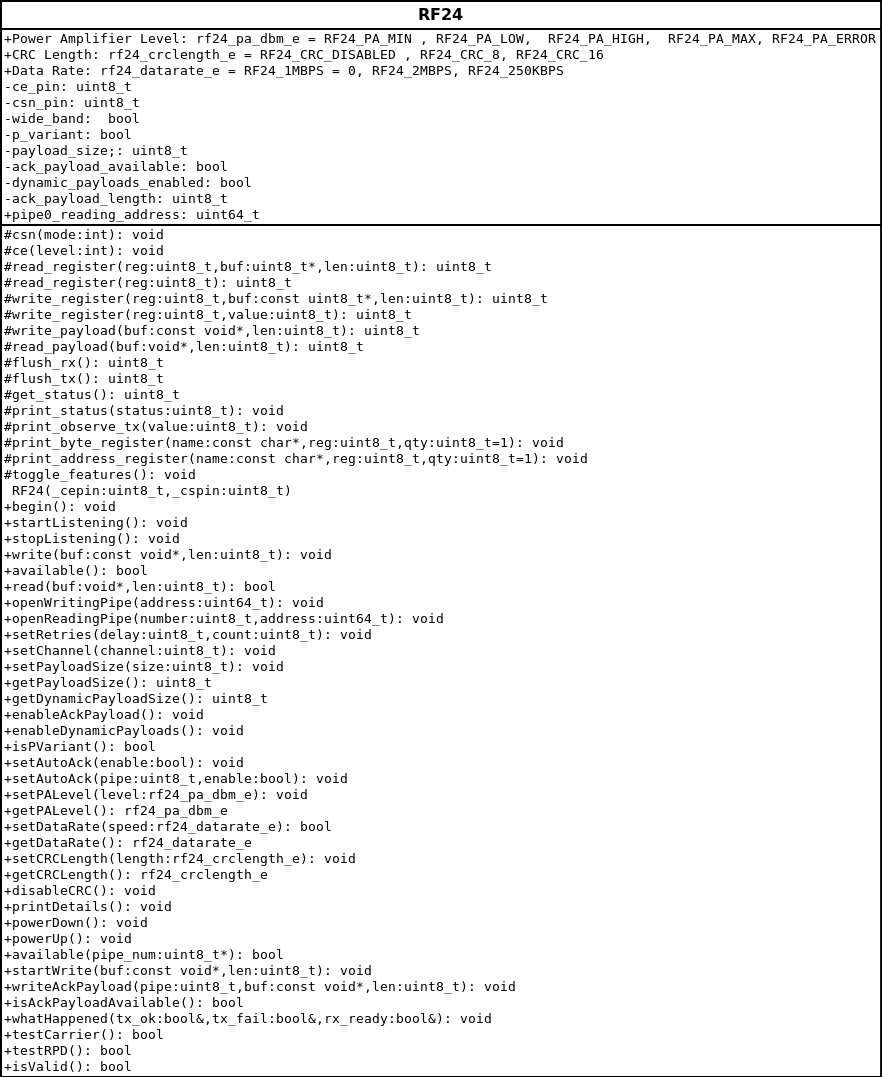
\includegraphics[width=\linewidth]{../../Imagens/RF24_class.png}
    \caption{Diagrama da Classe RF24} %% TODO certificar se realmente é uma WBS!!!
    \label{RF24_ClassDiag}
  \end{figure}

\section{Estrutura Analítica do Projeto}
  \begin{figure}[!htb] %% TODO certificar se realmente é uma WBS!!!
    \centering
    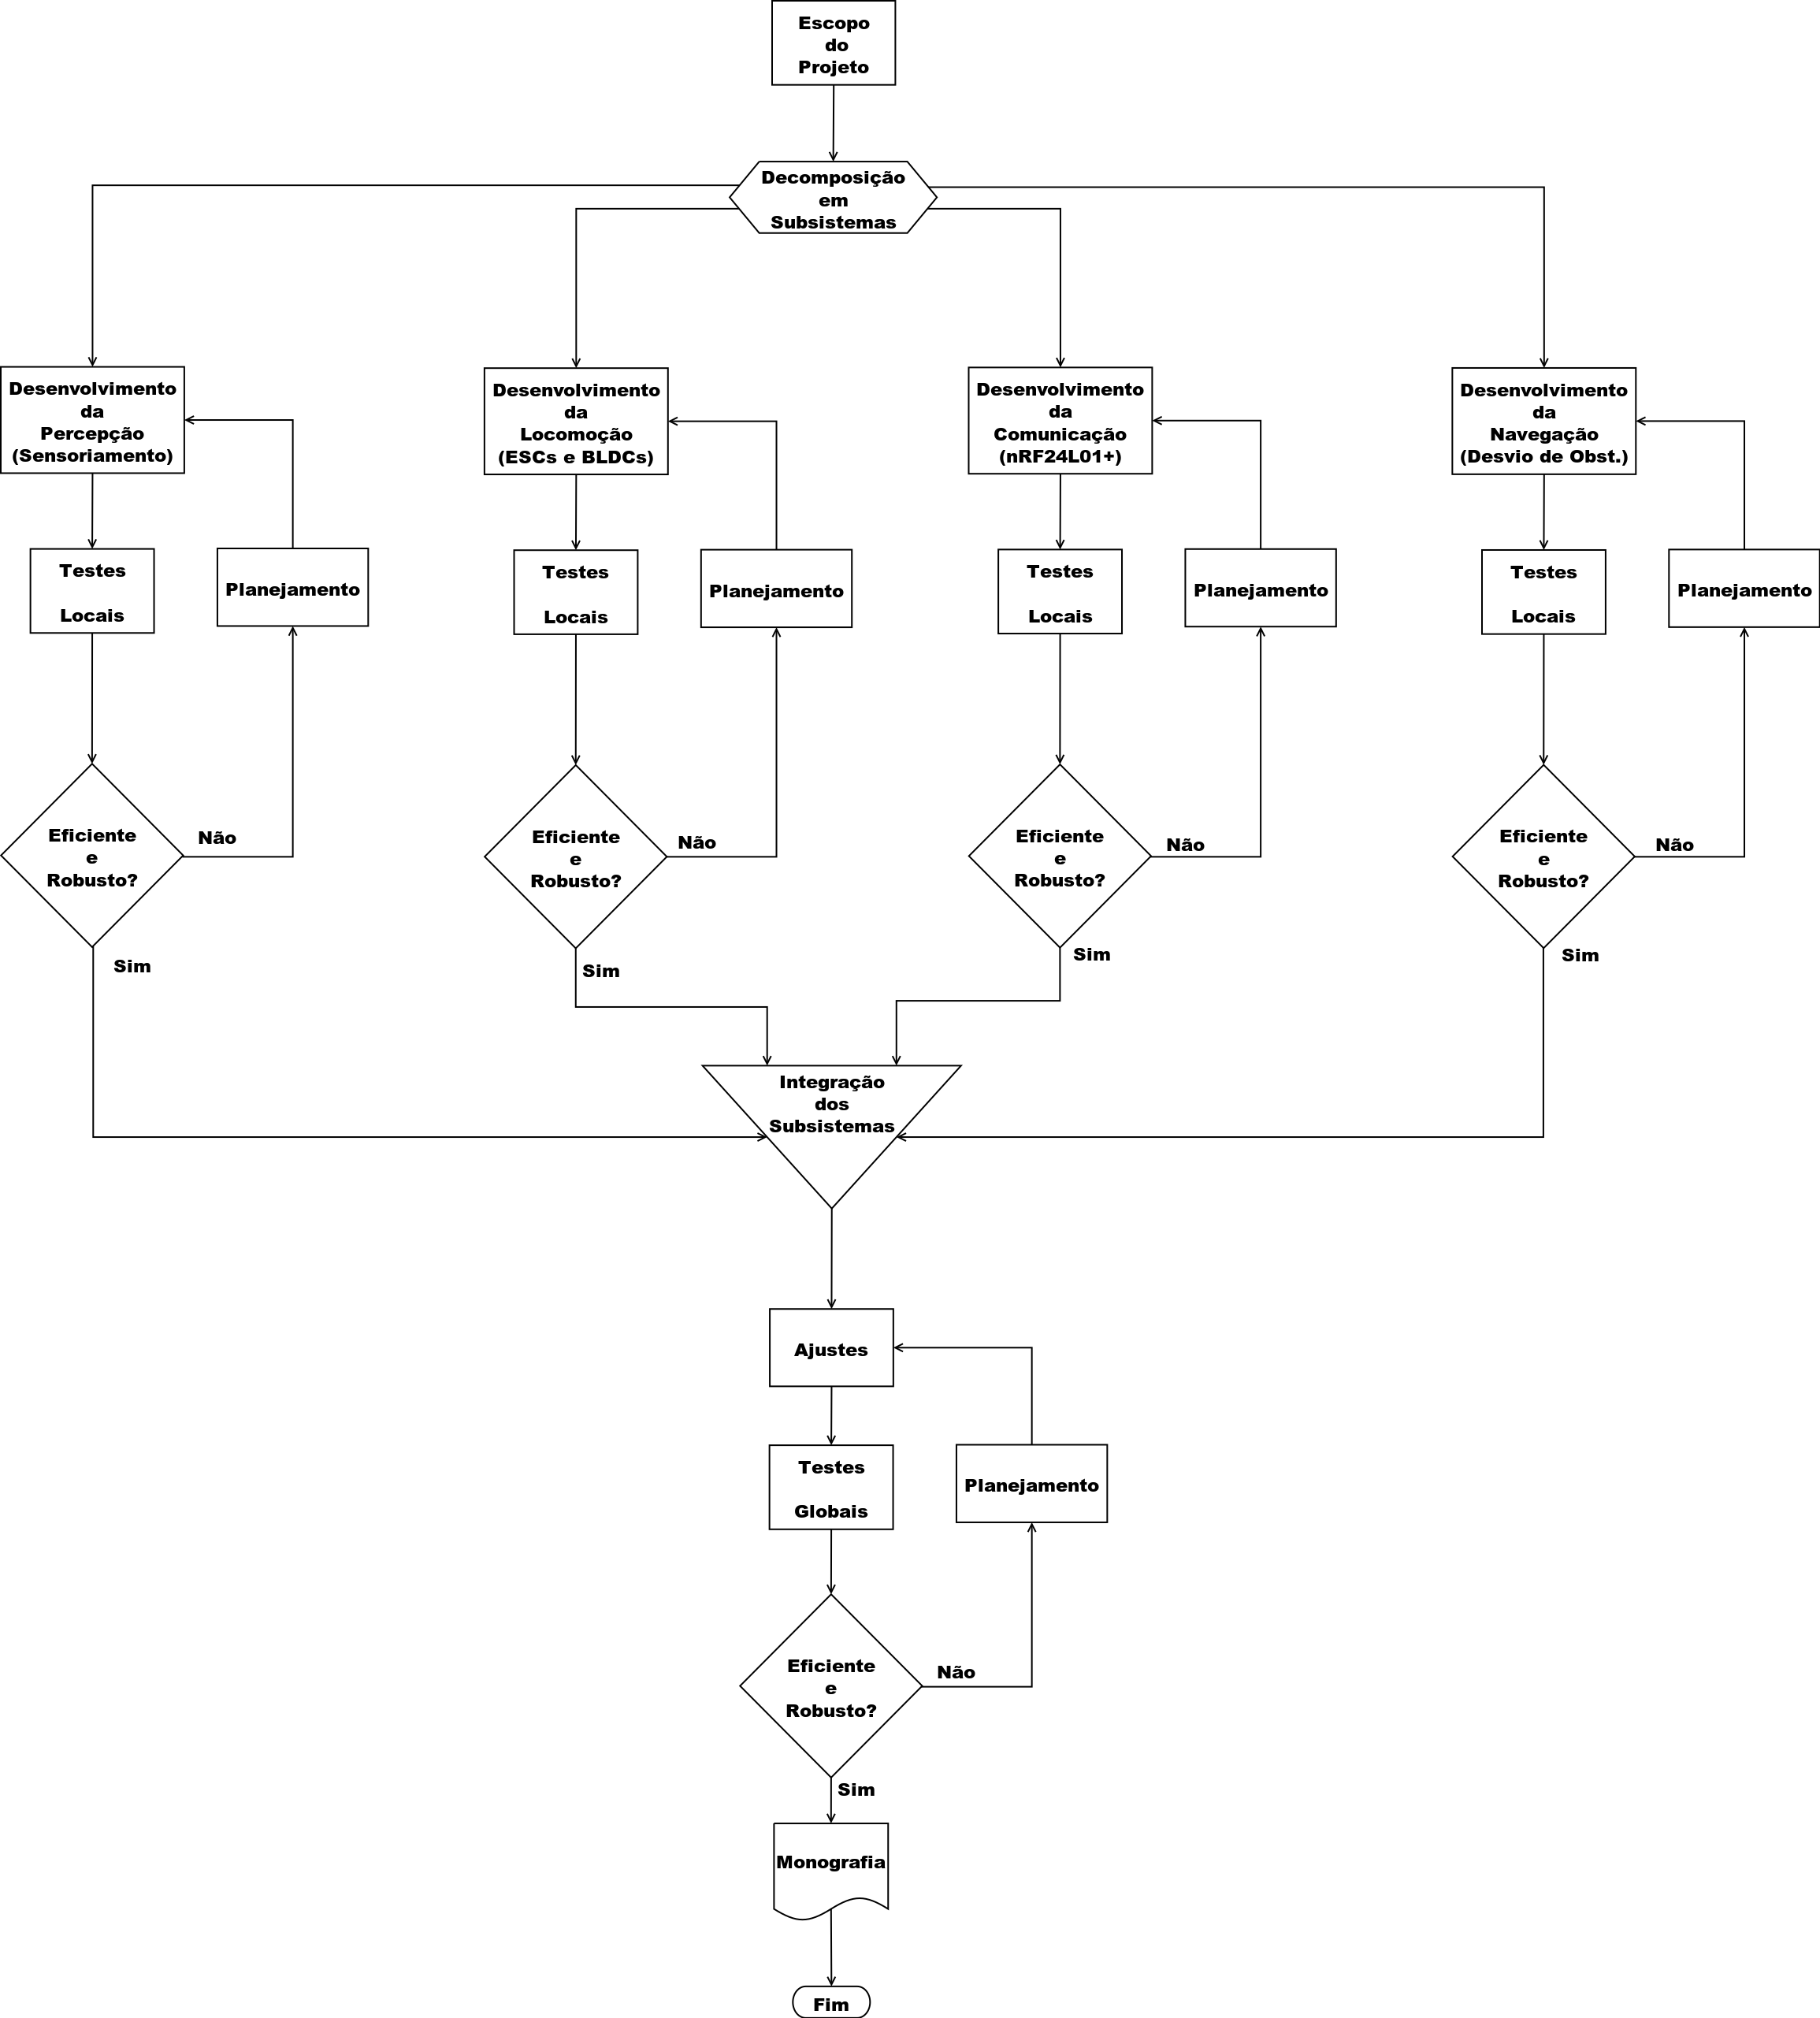
\includegraphics[width=\linewidth]{../../Imagens/WBS.png}
    \caption{Estrutura Analítica do Projeto} %% TODO certificar se realmente é uma WBS!!!
    \label{WBS}
  \end{figure}
  
\section{Esquemático do Robô}
  \begin{figure}[!htb]
    \centering
    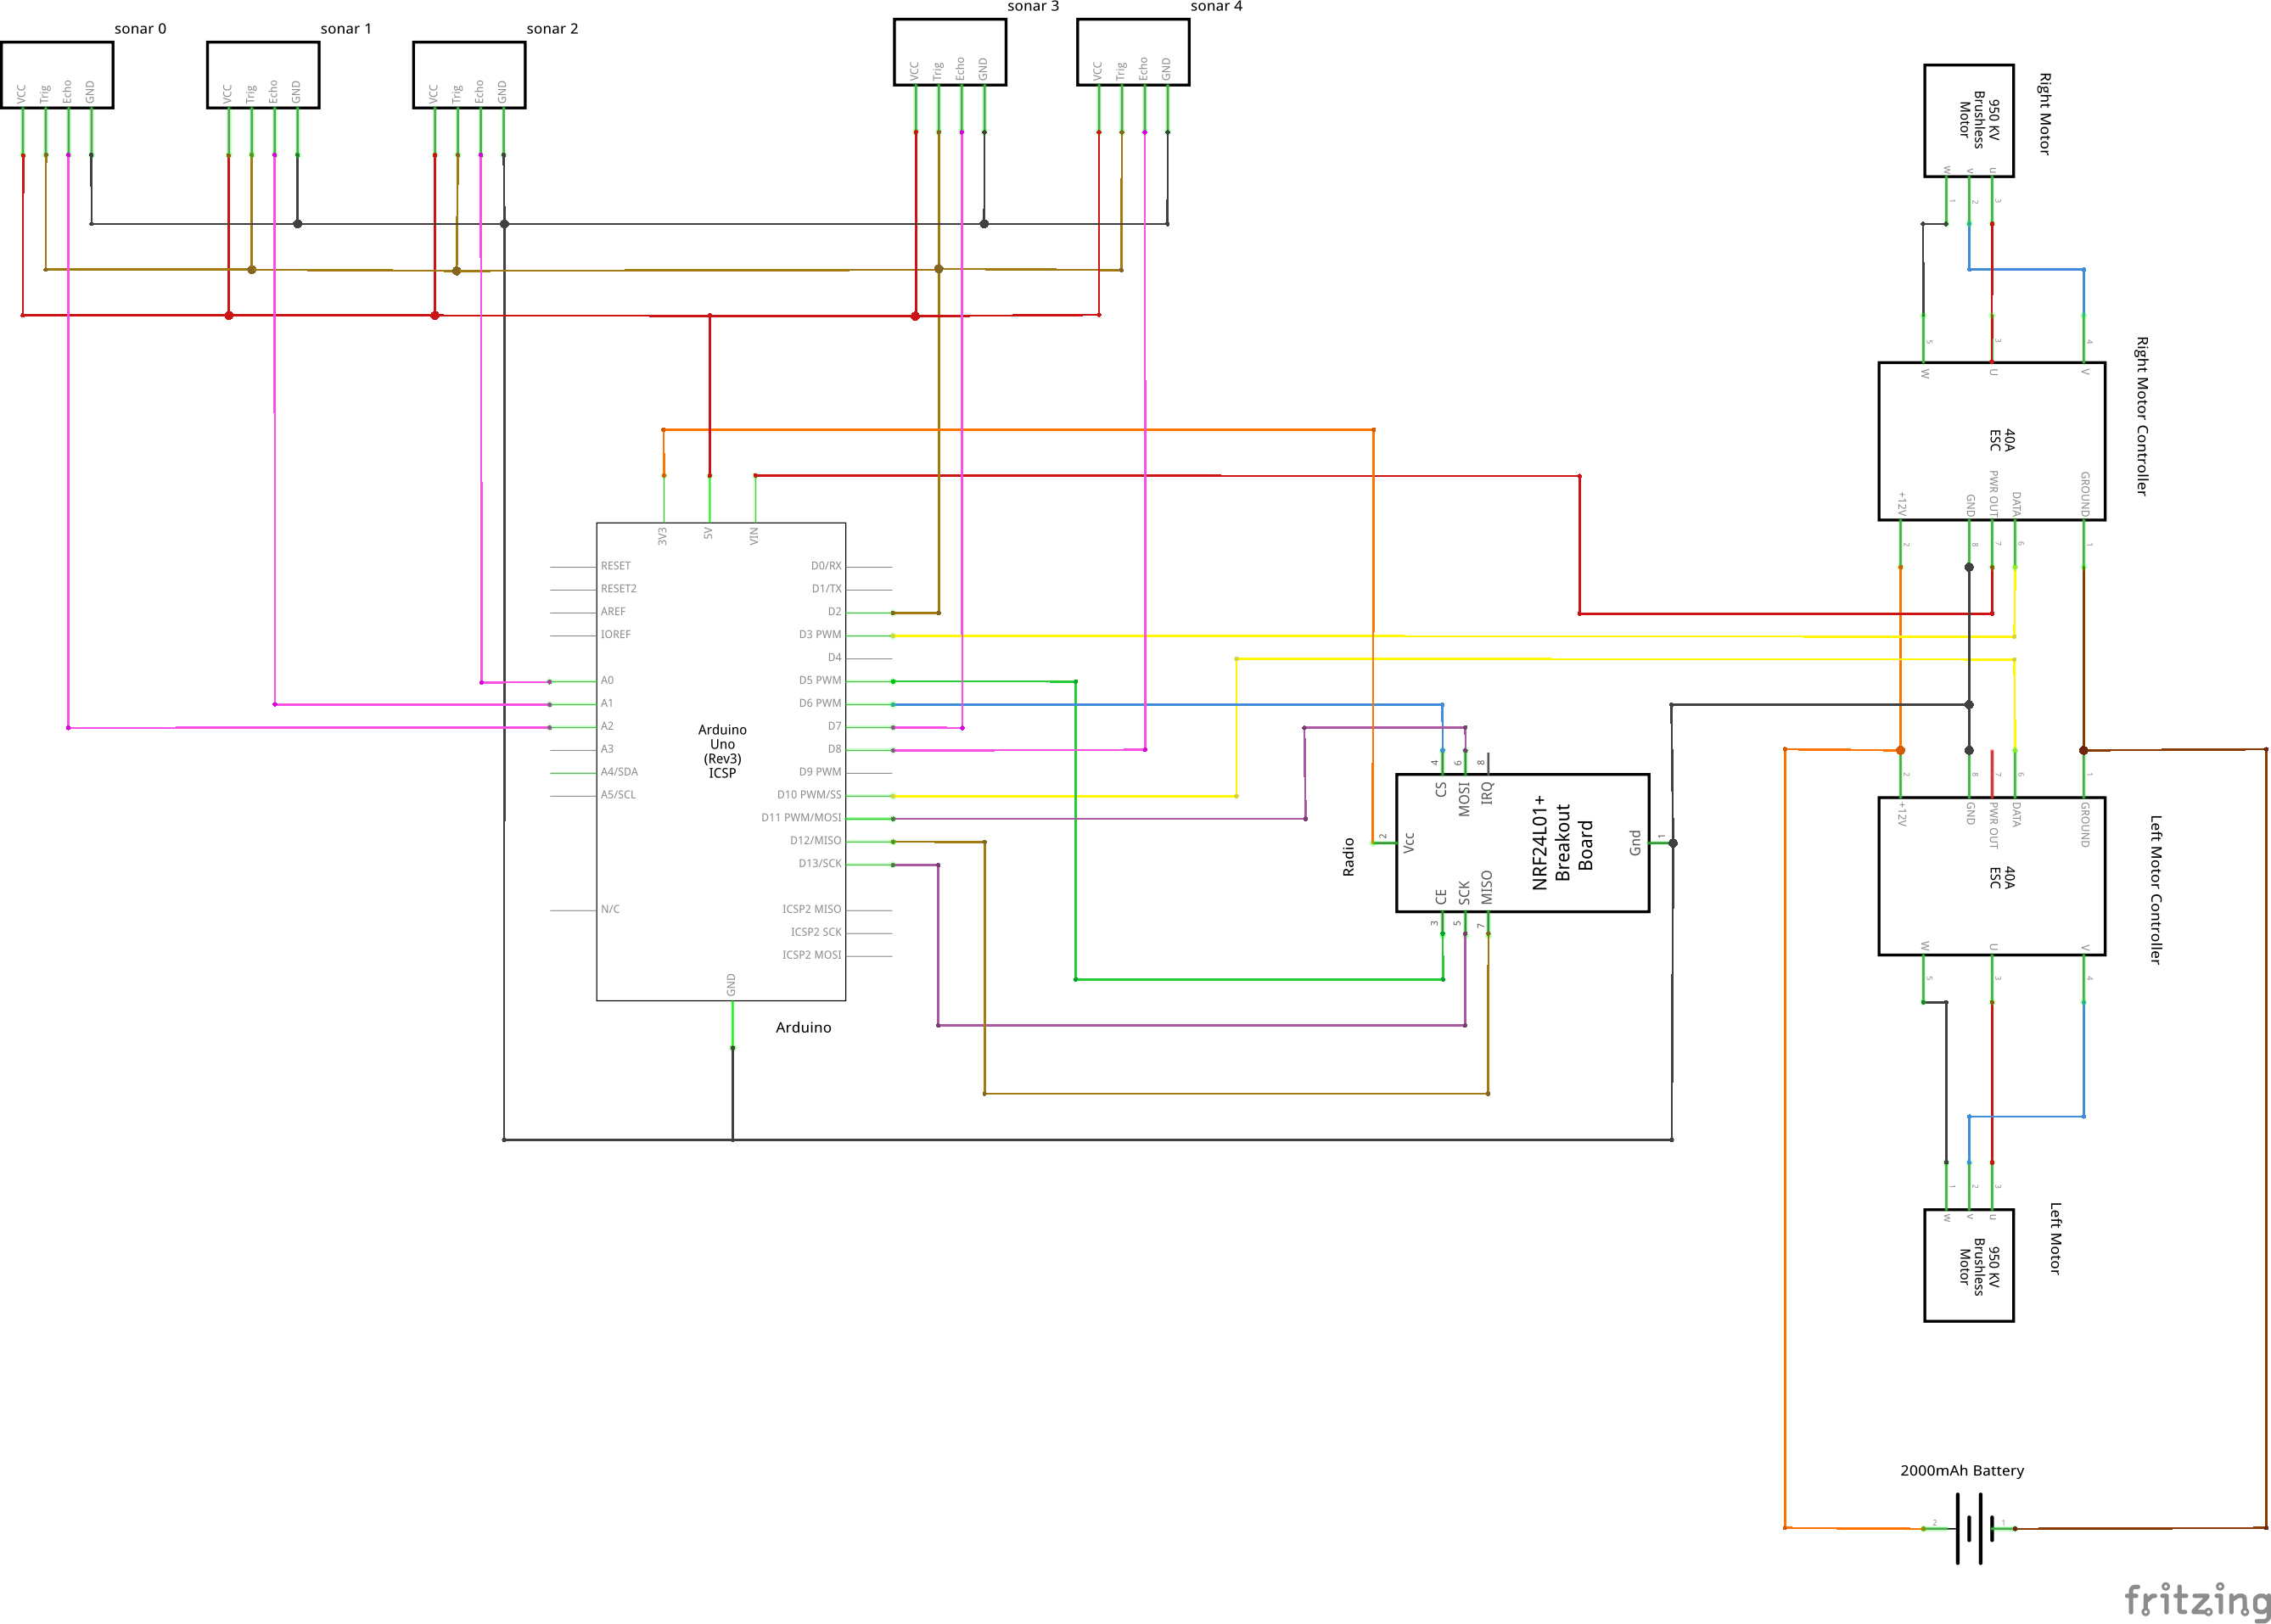
\includegraphics[width=\linewidth]{../../Imagens/robot_schem.png}
    \caption{Diagrama Elétrico} %% TODO: é um bom nome??
    \label{fritzing}
  \end{figure}
  
\section{Tabela}

\begin{table}[!htb]
\centering
\caption{}
\label{IA}
\begin{tabular}{|ccccc|c|}
\hline
{\color[HTML]{00009B} \textbf{$USS_0$}} & {\color[HTML]{00009B} \textbf{$USS_1$}} & {\color[HTML]{00009B} \textbf{$USS_2$}} & 
{\color[HTML]{00009B} \textbf{$USS_3$}} & {\color[HTML]{00009B} \textbf{$USS_4$}} & {\color[HTML]{FE0000} \textbf{Action}} \\ 
\hline
{\color[HTML]{00009B} 0}                                     & {\color[HTML]{00009B} 0}                                    & {\color[HTML]{00009B} 0}                                    & {\color[HTML]{00009B} 0}                                    & {\color[HTML]{00009B} 1}                                    & {\color[HTML]{FE0000} $E_L$}                                     \\ \hline
{\color[HTML]{00009B} 0}                                     & {\color[HTML]{00009B} 0}                                    & {\color[HTML]{00009B} 0}                                    & {\color[HTML]{00009B} 1}                                    & {\color[HTML]{00009B} 0}                                    & {\color[HTML]{FE0000} $E_M$}                                     \\ \hline
{\color[HTML]{00009B} 0}                                     & {\color[HTML]{00009B} 0}                                    & {\color[HTML]{00009B} 0}                                    & {\color[HTML]{00009B} 1}                                    & {\color[HTML]{00009B} 1}                                    & {\color[HTML]{FE0000} $E_M$}                                     \\ \hline
{\color[HTML]{00009B} 0}                                     & {\color[HTML]{00009B} 0}                                    & {\color[HTML]{00009B} 1}                                    & {\color[HTML]{00009B} 0}                                    & {\color[HTML]{00009B} 0}                                    & {\color[HTML]{FE0000} $E_F$}                                     \\ \hline
{\color[HTML]{00009B} 0}                                     & {\color[HTML]{00009B} 0}                                    & {\color[HTML]{00009B} 1}                                    & {\color[HTML]{00009B} 0}                                    & {\color[HTML]{00009B} 1}                                    & {\color[HTML]{FE0000} $E_F$}                                     \\ \hline
{\color[HTML]{00009B} 0}                                   & {\color[HTML]{00009B} 0}                                    & {\color[HTML]{00009B} 1}                                    & {\color[HTML]{00009B} 1}                                    & {\color[HTML]{00009B} 0}                                    & {\color[HTML]{FE0000} $E_F$}                                     \\ \hline
{\color[HTML]{00009B} 0}                                    & {\color[HTML]{00009B} 0}                                  & {\color[HTML]{00009B} 1}                                    & {\color[HTML]{00009B} 1}                                    & {\color[HTML]{00009B} 1}                                    & {\color[HTML]{FE0000} $E_F$}                                     \\ \hline
{\color[HTML]{00009B} 0}                                     & {\color[HTML]{00009B} 1}                                    & {\color[HTML]{00009B} 0}                                  & {\color[HTML]{00009B} 0}                                    & {\color[HTML]{00009B} 0}                                    & {\color[HTML]{FE0000} $D_M$}                                     \\ \hline
{\color[HTML]{00009B} 0}                                    & {\color[HTML]{00009B} 1}                                    & {\color[HTML]{00009B} 0}                                    & {\color[HTML]{00009B} 0}                                 & {\color[HTML]{00009B} 1}                                    & {\color[HTML]{FE0000} $D_M$}                                     \\ \hline
{\color[HTML]{00009B} 0}                                    & {\color[HTML]{00009B} 1}                                    & {\color[HTML]{00009B} 0}                                    & {\color[HTML]{00009B} 1}                                    & {\color[HTML]{00009B} 0}                                    & {\color[HTML]{FE0000} $E_F$}                                     \\ \hline
{\color[HTML]{00009B} 0}                                    & {\color[HTML]{00009B} 1}                                    & {\color[HTML]{00009B} 0}                                    & {\color[HTML]{00009B} 1}                                    & {\color[HTML]{00009B} 1}                                    & {\color[HTML]{FE0000} $E_M$}                                  \\ \hline
{\color[HTML]{00009B} 0}                                     & {\color[HTML]{00009B} 1}                                    & {\color[HTML]{00009B} 1}                                    & {\color[HTML]{00009B} 0}                                    & {\color[HTML]{00009B} 0}                                    & {\color[HTML]{FE0000} $D_F$}                                     \\ \hline
{\color[HTML]{00009B} 0}                                     & {\color[HTML]{00009B} 1}                                    & {\color[HTML]{00009B} 1}                                    & {\color[HTML]{00009B} 0}                                    & {\color[HTML]{00009B} 1}                                    & {\color[HTML]{FE0000} $E_F$}                                     \\ \hline
{\color[HTML]{00009B} 0}                                     & {\color[HTML]{00009B} 1}                                    & {\color[HTML]{00009B} 1}                                    & {\color[HTML]{00009B} 1}                                    & {\color[HTML]{00009B} 0}                                    & {\color[HTML]{FE0000} $E_F$}                                     \\ \hline
{\color[HTML]{00009B} 0}                                     & {\color[HTML]{00009B} 1}                                    & {\color[HTML]{00009B} 1}                                    & {\color[HTML]{00009B} 1}                                    & {\color[HTML]{00009B} 1}                                    & {\color[HTML]{FE0000} $E_F$}                                     \\ \hline
{\color[HTML]{00009B} 1}                                     & {\color[HTML]{00009B} 0}                                    & {\color[HTML]{00009B} 0}                                    & {\color[HTML]{00009B} 0}                                    & {\color[HTML]{00009B} 0}                                    & {\color[HTML]{FE0000} $D_L$}                                     \\ \hline
{\color[HTML]{00009B} 1}                                     & {\color[HTML]{00009B} 0}                                    & {\color[HTML]{00009B} 0}                                    & {\color[HTML]{00009B} 0}                                    & {\color[HTML]{00009B} 1}                                    & {\color[HTML]{FE0000} Frente}                                     \\ \hline
{\color[HTML]{00009B} 1}                                     & {\color[HTML]{00009B} 0}                                    & {\color[HTML]{00009B} 0}                                    & {\color[HTML]{00009B} 1}                                    & {\color[HTML]{00009B} 0}                                    & {\color[HTML]{FE0000} $E_M$}                                     \\ \hline
{\color[HTML]{00009B} 1}                                     & {\color[HTML]{00009B} 0}                                    & {\color[HTML]{00009B} 0}                                    & {\color[HTML]{00009B} 1}                                    & {\color[HTML]{00009B} 1}                                    & {\color[HTML]{FE0000} $E_M$}                                     \\ \hline
{\color[HTML]{00009B} 1}                                     & {\color[HTML]{00009B} 0}                                    & {\color[HTML]{00009B} 1}                                    & {\color[HTML]{00009B} 0}                                    & {\color[HTML]{00009B} 0}                                    & {\color[HTML]{FE0000} $D_F$}                                     \\ \hline
{\color[HTML]{00009B} 1}                                     & {\color[HTML]{00009B} 0}                                    & {\color[HTML]{00009B} 1}                                    & {\color[HTML]{00009B} 0}                                    & {\color[HTML]{00009B} 1}                                    & {\color[HTML]{FE0000} $E_F$}                                     \\ \hline
{\color[HTML]{00009B} 1}                                     & {\color[HTML]{00009B} 0}                                    & {\color[HTML]{00009B} 1}                                    & {\color[HTML]{00009B} 1}                                    & {\color[HTML]{00009B} 0}                                    & {\color[HTML]{FE0000} $E_F$}                                     \\ \hline
{\color[HTML]{00009B} 1}                                     & {\color[HTML]{00009B} 0}                                    & {\color[HTML]{00009B} 1}                                    & {\color[HTML]{00009B} 1}                                    & {\color[HTML]{00009B} 1}                                    & {\color[HTML]{FE0000} $E_F$}                                     \\ \hline
{\color[HTML]{00009B} 1}                                     & {\color[HTML]{00009B} 1}                                    & {\color[HTML]{00009B} 0}                                    & {\color[HTML]{00009B} 0}                                    & {\color[HTML]{00009B} 0}                                    & {\color[HTML]{FE0000} $D_M$}                                     \\ \hline
{\color[HTML]{00009B} 1}                                     & {\color[HTML]{00009B} 1}                                    & {\color[HTML]{00009B} 0}                                    & {\color[HTML]{00009B} 0}                                    & {\color[HTML]{00009B} 1}                                    & {\color[HTML]{FE0000} $D_M$}                                     \\ \hline
{\color[HTML]{00009B} 1}                                     & {\color[HTML]{00009B} 1}                                    & {\color[HTML]{00009B} 0}                                    & {\color[HTML]{00009B} 1}                                    & {\color[HTML]{00009B} 0}                                    & {\color[HTML]{FE0000} $D_M$}                                     \\ \hline
{\color[HTML]{00009B} 1}                                     & {\color[HTML]{00009B} 1}                                    & {\color[HTML]{00009B} 0}                                    & {\color[HTML]{00009B} 1}                                    & {\color[HTML]{00009B} 1}                                    & {\color[HTML]{FE0000} Frente}                                     \\ \hline
{\color[HTML]{00009B} 1}                                     & {\color[HTML]{00009B} 1}                                    & {\color[HTML]{00009B} 1}                                    & {\color[HTML]{00009B} 0}                                    & {\color[HTML]{00009B} 0}                                    & {\color[HTML]{FE0000} $D_F$}                                     \\ \hline
{\color[HTML]{00009B} 1}                                     & {\color[HTML]{00009B} 1}                                    & {\color[HTML]{00009B} 1}                                    & {\color[HTML]{00009B} 0}                                    & {\color[HTML]{00009B} 1}                                    & {\color[HTML]{FE0000} $D_F$}                                     \\ \hline
{\color[HTML]{00009B} 1}                                     & {\color[HTML]{00009B} 1}                                    & {\color[HTML]{00009B} 1}                                    & {\color[HTML]{00009B} 1}                                    & {\color[HTML]{00009B} 0}                                    & {\color[HTML]{FE0000} $D_F$}                                     \\ \hline
{\color[HTML]{00009B} 1}                                     & {\color[HTML]{00009B} 1}                                    & {\color[HTML]{00009B} 1}                                    & {\color[HTML]{00009B} 1}                                    & {\color[HTML]{00009B} 1}                                    & {\color[HTML]{FE0000} $E_F$}                                    \\ \hline

\end{tabular}
\end{table}

\section{Fluxograma da Rotina de Desvio de Obstáculos}
  \begin{figure}[!htb]
    \centering
    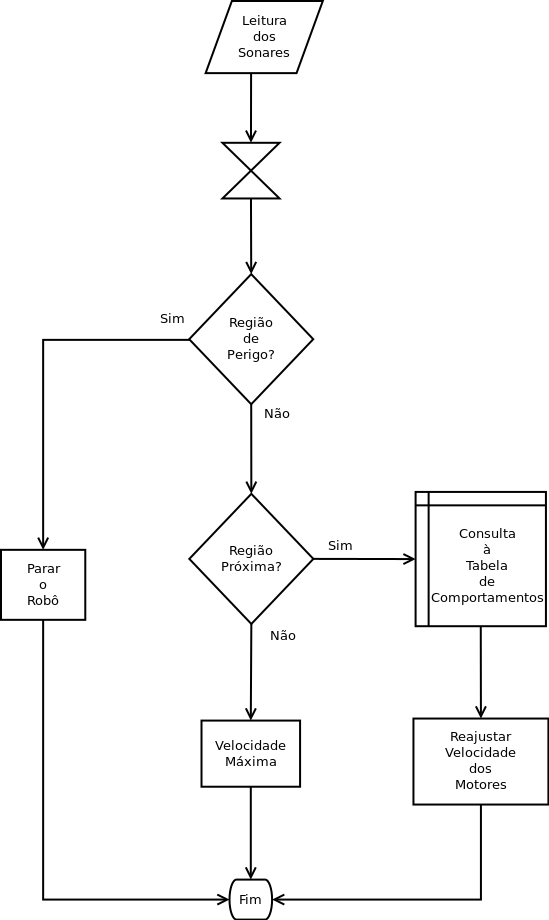
\includegraphics[width=0.8 \linewidth]{../../Imagens/ObstAvoid.png}
    \caption{Fluxograma da Rotina de Desvio de Obstáculos}
    \label{ObstAvoid}
  \end{figure}